\begin{savequote}
Simplicity is the ultimate sophistication.
\qauthor{Leonardo da Vinci}
\end{savequote}

\chapter[Feature Selection for NVC Regression]{Feature Selection for NVC Regression}
\label{ChapterFeatureSelection}

\thesiscomment{WHAT we do}

\thesiscomment{HOW we do it}

\thesiscomment{RESULTS, IMPACT and NOVELTY}

%The previous chapter described an automatic system for \ac{NVC} regression. 
The features used in the two previous chapters were extracted based on distances between pairs of tracker positions. These features encoded local deformations of the face, with each feature component corresponding to a specific, local area. 
%The features were used to build a model of \ac{NVC} signals for recognition based on unseen samples. 
Expression of emotions or \ac{NVC} signals only involve part of the face but the features also encode areas of the face that are not involved in a specific \ac{NVC} expression. Therefore, the feature data contains irrelevant information. Redundant information is also present in the algorithmic features, with tracker motions in a local area of the face often being closely coupled. Training based on features that are largely irrelevant leads to over-fitting, in which the \ac{NVC} model is based on noise or incorrect features, rather than modelling the true underlying pattern. This results in poor generalisation and poor performance. This can be addressed by various means, including \featureGeneration that is focused on the task at hand, or by feature selection. 

Feature selection is the process of determining the relevance of features for a \ac{ML} task. Using a smaller subset of relevant features reduces the computational complexity of \ac{ML}. As the relevance of each feature is computed, this can give an insight to how \ac{NVC} is expressed. Feature selection provides a way to find associations between \ac{NVC} signals, relevant feature components and the associated areas of the face. Feature selection is a broad discipline with many approaches.
Features are either assigned a relevance weight or a subset of relevant features is found. This chapter uses an existing wrapper based approach which determines which subset of features is relevant. The selected feature subset can then be applied to \ac{NVC} recognition and the performance change can be evaluated.

An \ac{NVC} signal specific feature selection is computed for each culture. The performance contribution of each feature component is also evaluated. This results in a set of feature relevance weights for each \ac{NVC} signal. The feature weights can be visualised to show the involvement of facial areas in the expression of \ac{NVC} in an intuitive manner. This is based on segmenting a face using Voronoi tessellation around the position of trackers. Voronoi tessellation segments an image into cells based around seed positions; each point in the space is assigned to a cell based on the nearest seed position. This visualisation can either be used to check if the relevant facial areas conform to our expectation, or provide an indication as to the areas used by the automatic system. This in turn may provide clues as to human \ac{NVC} perception, although facial areas used in human perception of emotion may differ from an automatic approach.

The main contributions of this chapter are:

\begin{itemize}
 \item A method of feature selection to select subset of features that are relevant for \ac{NVC} recognition.
 \item A method of visualisation of the relevant features that is easy and intuitive to interpret.
\end{itemize}

The next section provides an overview of relevant existing research. Section \ref{SectionSbeFeatureSelection} discusses feature selection for the purposes of improving performance.

\section{Related Research}

There are many approaches to feature selection, which vary in performance, computational cost and restrictions on the type of input data. There are three general types of feature selection (see Saeys \etal for a review \cite{Saeys2007}):

\begin{itemize}
 \item filter methods, that consider feature components either individually or in groups, but do not consider the \ac{ML} method used to make the final prediction. This scales to large sets of features. These methods do not consider effect of the \ac{ML} method and may ignore the effects of combining groups of features.
 \item wrapper methods, that consider sets of features in conjunction with an \ac{ML} method. They do consider groups of features in context with \ac{ML} but they tend to be computationally intensive, they are classifier specific and are prone to over fitting.
 \item embedded methods, which are combined with \ac{ML} methods to select features. This makes the feature selection methodology and results specific to the \ac{ML} method used.
\end{itemize}

Existing papers that use feature selection for facial analysis will now be discussed. The use of an embedded feature selection, such as a boosting classifier, can be used to weight a set of features based on relevance. This feature subset can then be used by a second, more sophisticated classifier. This approach was used by Valstar \cite{Valstar2006} to select shape features by Gentleboost, and Petridis and Pantic \cite{Petridis2008} used Adaboost to select relevant audio and visual features. However, performing feature selection in this way, assumes there is similarity in the optimal set of features for both methods, which might not be the case. Yang \etal \cite{Yang2009} propose a feature selection method based on rough set theory on audio visual features. This avoids discretisation of feature values, as required by Adaboost, which may result in a loss of information. Filter based feature selection appears to have been largely avoided, probably because the number of feature components in the original feature vector is relatively low (usually thousands of feature components at most), and the interaction between features is often significant for emotion and \ac{NVC} recognition.

Wrapper based methods include randomised feature selection approaches such as simulated annealing and genetic approaches, but these have not been popular in facial analysis. Deterministic wrapper based approaches have been applied to emotion recognition: Grimm \cite{Grimm2007} used \ac{SFS} to isolate relevant audio features. This method begins with an empty set and incrementally adds features that produce the greatest performance increase, in a greedy fashion. An alternative, called \acf{SBE}, is to start with a full set of features and incrementally eliminate features that result in the best performance \cite{Kittler1978}. The \ac{SBE} approach was used by el Kaliouby and Robinson \cite{ElKaliouby2004} to find the most relevant geometric features.

There are several existing papers that identify which features have been selected for emotion or \ac{NVC} recognition, but it is less common to attempt to visualise which features have been selected. If features are shown, they are often visualised individually (e.g. \cite{Yang2009}), which can make comprehension of the overall distribution difficult. In experimental psychology, gaze patterns in perception have been visualised \cite{Jack2009}. Busso and Narayanan visualised areas of the face that were correlated with prosodic and vocal tract features for different emotions \cite{Busso2007}. It would be beneficial to have a method that is similar to these approaches for visualisation of feature selection results in a way that can be intuitively understood. 
%The next section will apply feature selection to the problem of \ac{NVC} recognition.

\section{\acs{SBE} Feature Selection}
\label{SectionSbeFeatureSelection}

%The previous chapter used geometric features to transform feature point tracking into a form that can be used by conventional \ac{ML} techniques. The geometric features (\textit{geometric-a}) are based on the distance between pairs of feature point trackers. However, this feature is likely to contain a great deal of redundant information. These features also contain noise from tracking drift and occasional occlusions. These noisy, redundant features result in a lower performance, as the regression model can have difficulty determining which features are relevant. This is addressed by using a technique to select the relevant features and remove those that are noisy or redundant. 
The approach used is a greedy \ac{SBE} of the features \cite{Kittler1978}. This section describes the method in detail and the resulting performance impact. 
%The advantage of \ac{SBE} is that interactions between subsets of variables are exploited. The main disadvantages of the method are possible over-fitting and a high computational cost.
Backward searching was thought to be preferable to forward searching because the interaction of features can be found and exploited. Forward search, particularly in the first few iterations, adds features without the benefit of other complimentary features. In contrast, a backward search allows irrelevant features to be eliminated while retaining features that contain complementary information. Also, it is possible to accelerate the backward search by removing more than one feature at each iteration, which reduces the computational cost.
Some feature component subsets are more effective than others. Unfortunately, \ac{SBE} may not find a globally optimal feature subset. If all possible feature subsets are considered as a space, \ac{SBE} performs a gradient descent to minimise error. 
%This type of search is not guaranteed to find a global optimum. 
% Alternative approaches, such as a forward-backwards search and exhaustive search were not used because they require higher computational resources and it is difficult to find approximations that reduce the computational cost to a practical level. The next section describes feature selection by \ac{SBE}.

\subsection{Method}

Feature selection occurs within a person independent, cross validation framework. There are eight folds in cross validation, resulting in eight different partitionings of seen and unseen data sets. Feature selection is applied to the seen data of a specific cross validation fold, to determine a relevant feature subset. \ac{SVR} is then applied to the feature subset to produce a model suitable for prediction.

%\begin{figure}[tb]
%\centering
%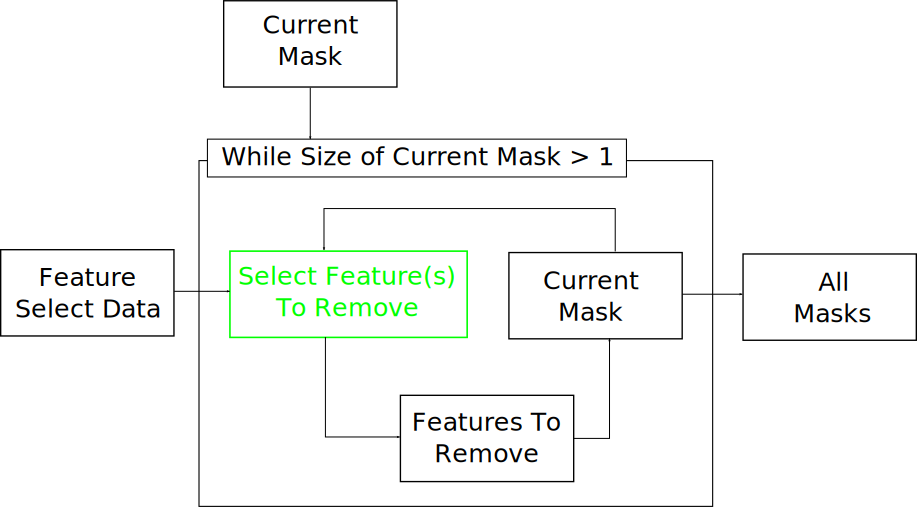
\includegraphics[width = 0.7 \columnwidth]{featureselection/feature-select.pdf}
%\caption{High level overview of feature selection. Features are selected by a greedy backward elimination, beginning with a %feature set that contains all possible features. The feature set at each stage is stored for later use. The detail of the ``select features for removal'' block is shown in Figure \ref{FigureFeaturesToRemove}.}
%\label{FigureFeatureSelectOverview}
%\end{figure}

\begin{algorithm}
\scriptsize 
\lstset{language=Python}
\begin{lstlisting}[frame=single]
def PerformFeatureSelection(data, labels):

   #The current mask begins with every feature enabled
   currentMask = np.ones((data.shape[1]), dtype=np.bool)

   #For storing the intermediate steps during feature selection
   allMasks = []

   #While more than one feature remains in the current mask
   while currentMask.sum() > 1:

      #Evaluate which features to remove
      toRemove = EvaluateRemainingFeatures(currentMask, data, labels)

      #Update the current mask and remove features
      for featToRemove in toRemove:
         currentMask[featToRemove[1]] = False

      #Store mask for later analysis
      allMasks.append(currentMask)

   return allMasks
\end{lstlisting}
\normalsize
\caption{Features are selected by a greedy backward elimination, beginning with a feature set that contains all possible features. The feature set at each stage is stored for later use. The algorithm is expressed as Python 2.7 code. The function \textit{EvaluateRemainingFeatures} is defined in Algorithm \ref{AlgFeaturesToRemove}.}
\label{AlgFeatureSelectOverview}
\end{algorithm}

The procedure for \acs{SBE} is shown in Algorithm \ref{AlgFeatureSelectOverview}. %Figure \ref{FigureFeatureSelectOverview}.
The search begins with a current set $\currentFeatureSet = \{1...\numFeatures\}$ which is initialised to include all possible feature components. The components to be removed from $\currentFeatureSet$ at each iteration is then determined. The current set $\currentFeatureSet$ is then updated and the process continues until the current set $\currentFeatureSet$ is empty. For the large number of components, it is too time consuming to remove components at a rate of 1 per iteration. To accelerate the process, multiple feature components are removed nearer the start of the \ac{SBE} process. As the number of components in the current set approaches zero, the rate of feature elimination returns to the standard 1 feature component per iteration. This produces a significant speed increase, but risks the removal of non-optimal components and this may result in a sub-optimal final feature set. The number of feature components removed from the current feature set at each iteration is denoted $\numToRemoveInMask$. This depends on the number of feature components $\numFeaturesInMask$ in the current set $\currentFeatureSet$ as follows:

\begin{gather}
\label{EquationNumFeaturesToRemove}
\numToRemoveInMask = \begin{cases}
200 : \numFeaturesInMask > 1000 \\
100 : \numFeaturesInMask > 400, \numFeaturesInMask \le 1000 \\
1 : \numFeaturesInMask \le 400
\end{cases}
\end{gather}

These thresholds were based on an intuitive expectation that only a small subset of features are required for accurate recognition.

%\begin{figure}[tb]
%\centering
%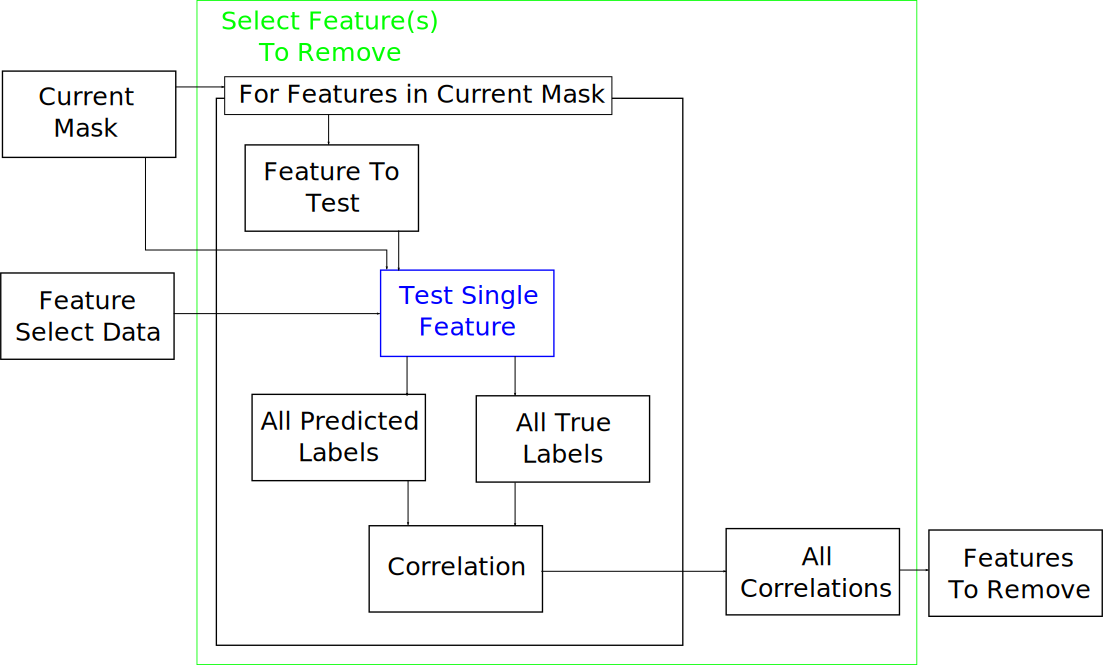
\includegraphics[width = 0.9 \columnwidth]{featureselection/select-features-to-remove.pdf}
%\caption{Each feature in the current feature set is tested. The features that cause the best performance are retained and the %features that worsen performance are preferred for removal. The detail for block marked ``test single feature'' is shown in Figure \ref{FigureTestSingleFeature}}
%\label{FigureFeaturesToRemove}
%\end{figure}

\begin{algorithm}
\scriptsize 
\lstset{language=Python}
\begin{lstlisting}[frame=single]
def EvaluateRemainingFeatures(mask, data, labels):

   #Determine how many components to remove, based on the mask
   numToRemove = CalcNumToRemove(mask.sum()) 

   #Initalise an empty list, based on the number of components in the mask
   scores = [None for count in range(mask.sum())] 

   #For each remaining component in the mask
   for count, featNum in enumerate(np.where(mask == True)[0]):

      #Create a test mask with a single component disabled
      testMask = np.copy(currentMask)
      testMask[featNum] = False

      #Evaluate the perfomance of the test mask and store the score
      scores[count] = (TestPerf(data[:, testMask], labels), featNum)

   #Return a list of features to remove
   scores.sort()
   scores.reverse()
   return scores[:numToRemove]
\end{lstlisting}
\normalsize
\caption{Each feature in the current feature set is tested. The features that cause the best performance are retained and the features that worsen performance are preferred for removal. The function \textit{TestPerf} is defined in Algorithm \ref{AlgTestSingleFeature}.}
\label{AlgFeaturesToRemove}
\end{algorithm}

To find an appropriate subset of features for removal from the current feature set, the contribution of each feature component needs to be assessed. An overview of this process is shown in Algorithm \ref{AlgFeaturesToRemove}. %Figure \ref{FigureFeaturesToRemove}. 
Each feature component in the current feature set $\currentFeatureSet$ is selected as the test component and the performance impact of the removal of the component is evaluated. The features are then prioritised, with the feature components resulting in the lowest performance preferred for removal. This process becomes progressively faster as the current feature set becomes smaller.

%\begin{figure}[tb]
%\centering
%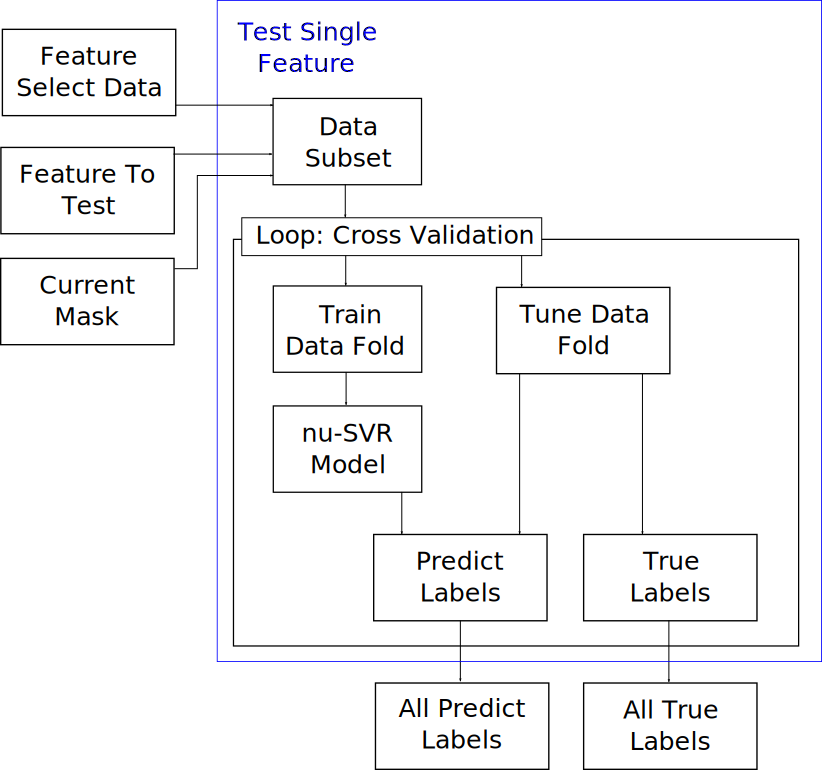
\includegraphics[width = 0.7 \columnwidth]{featureselection/test-single-feature.pdf}
%\caption{The feature being tested is temporarily removed from the feature set. The system is then tested to check what effect this has on overall performance. This is carried out in another inner, ``feature selection'' cross validation loop.}
%\label{FigureTestSingleFeature}
%\end{figure}

\begin{algorithm}
\scriptsize 
\lstset{language=Python}
\begin{lstlisting}[frame=single]
def TestPerf(maskedData, labels):

   #Prepare cross validation sets
   kf = cross_validation.KFold(len(maskedData), numFolds)

   #Create an empty list for predictions
   allPredictions = [] 
   allLabels = []

   for train, test in kf: #For each cross validation fold

      #Fit a regression model on the training data
      regressor.fit(maskedData[train,:], labels[train])

      #Store the predictions based on the test data
      allPredictions.extend(regressor.predict(maskedData[test,:])) 

      #Store the test labels in this fold
      allLabels.extend(labels[test]) 

   #Calculate the overall correlation of predictions and test labels
   return np.corrcoef(allPredictions, allLabels)[0,1]
\end{lstlisting}
\normalsize
\caption{Testing the performance of a test set of feature components. The regression can use any suitable method, but in this study $\nu$-SVR is used.}
\label{AlgTestSingleFeature}
\end{algorithm}

To test a specific feature component, regression models are trained and tested to assess the performance of the remaining feature components as shown in Algorithm \ref{AlgTestSingleFeature}. %Figure \ref{FigureTestSingleFeature}. 
A temporary set $\tempFeatureSet$ is created which creates a copy of the current set $\currentFeatureSet$ except for the removal of the test component $i$:

\begin{gather}
\tempFeatureSet = \{j: j \in \currentFeatureSet, j \ne i\}
\end{gather}

The feature data is split into cross validation folds. These ``feature selection'' folds are distinct from the ``system'' cross validation folds discussed earlier, so that each fold contains data from multiple human subjects.

This produces a series of sets $\{\currentFeatureSet^\numFeatures..\currentFeatureSet^1\}$ that correspond to each stage in the progressive removal of features. Each set contains a different number of feature components. The performance of the feature set on the unseen data can then be determined. The expectation is for an increase in performance as poor features are removed. As the \ac{SBE} process is nearing termination, some features that are critical to \ac{NVC} regression are removed and the performance sharply declines. The performance of the feature subset at each stage is evaluated and retained for later analysis.

Because this process results in multiple sets which are used to create multiple \ac{NVC} models, it is not obvious which feature set to use and how many feature components are optimal. Simply selecting the peak performance when evaluating feature sets on unseen data violates the separation of seen and unseen data. For simplicity, this section uses the feature set $\currentFeatureSet^{unseen}$ having the peak performance for unseen test data to determine the number of feature components. It is likely that different \ac{NVC} signals require a specific set of geometric features to be effective. Therefore, feature selection is computed for a specific \ac{NVC} category and using a specific culture's annotation data. The processing of test set $\tempFeatureSet$ has been parallelized in this implementation, resulting in a speed increase. The next section uses the set $\currentFeatureSet^{seen}$ having the highest performance on seen training data only.

\subsection{Results}
\label{SectionFeatureSelectionUnseenPeak}

\begin{figure}[tb]
\centering
\includegraphics[width = 0.7 \columnwidth]{featureselection/shuffle-gbr-think/shufflefs-reverse-GBR-thinking-3008.pdf}
\caption[The performance of the system progressively improves as backward feature selection eliminates poor features.]{The performance of the system progressively improves as backward feature selection eliminates poor features. The upper line shows the seen data, which is used in the feature selection algorithm. The lower line shows the performance of the unseen data. The unseen data corresponds to subject 3008.}
\label{FigureShuffleGbrThink}
\end{figure}

%\ac{SBE} feature selection is performed by progressively removing features based on their effect on \ac{NVC} regression performance. 
A typical plot of performance against the number of feature components in the subset is shown in Figure \ref{FigureShuffleGbrThink}. As expected, the performance of predicting unseen test data increases as features are removed until performance suffers a sharp decline. The far left starting point of the lower curve corresponds to the performance of the system discussed in the previous chapter (i.e. without feature selection). In this example, feature selection results in a significant increase in performance. A feature set containing between 10 to 275 features encompasses the highest performance, with the peak performance requiring only 10 features. This feature set is smaller than the terse $\frameFeature_{geometric-h}$ features (Section \ref{SectionGenerateHeuristic}). However, it is unlikely that this feature set will be effective for other non-\textit{thinking} \ac{NVC} regression. This can be a disadvantage because the \ac{SBE} method is \ac{NVC} category specific and a great deal of computation is required to retrain the system for a different \ac{NVC} signal.

The feature selection curves are relatively linear until approximately 400 features remain. This corresponds to the threshold in Equation \ref{EquationNumFeaturesToRemove}. The change in the curve behaviour at this point suggests that a different set of thresholds might result in a higher peak, although this was not investigated.

\begin{figure}[tb]
\centering
\includegraphics[width = 0.49 \columnwidth]{featureselection/shuffle-gbr-think/shufflefs-reverse-GBR-question-1011.pdf}
\includegraphics[width = 0.49 \columnwidth]{featureselection/shuffle-gbr-think/shufflefs-reverse-KEN-agree-1011.pdf}
\caption[Additional examples of performance increases as feature selection progresses.]{Additional examples of performance increases as feature selection progresses. The left plot shows GBR \textit{question} performance. The right plot shows KEN \textit{agree} performance. Both unseen data folds correspond to subject 1011.}
\label{FigureShuffleFeatureSelect}
\end{figure}

This pattern is repeated for most other \ac{NVC} categories and in different cultures. While almost every test fold subject benefits from the feature selection process, not all system cross validation folds yield the same level of performance increase. The left plot of Figure \ref{FigureShuffleFeatureSelect} shows an instance in which feature selection was not effective. The performance is low before feature selection begins, which might indicate a problem with the approach in recognizing this subject performing \textit{question} \ac{NVC} signals. The right curve shows typical feature selection behaviour in a different culture (KEN in this case). A typical gradual improvement in performance can be seen, as features are removed before a sharp decline.

%Use of unseen data to determine FS termination, which is kind of cheating, shuffled sets
\begin{table}[htb]
\centering
\caption[System performance with termination of features selection based on the peak of unseen performance.]{System performance with termination of features selection based on the peak of unseen performance. This violates the separation of training and test data but this shows the performance with an ideal termination point.}
\begin{tabular}{ | c | c | c | }
\hline
Area & NVC      & Terminate \\
     & Category & By Unseen \\
     &          & Peak \\
\hline
GBR & Agree & 0.588 \\
GBR & Question & 0.453 \\
GBR & Thinking & 0.617 \\
GBR & Understand & 0.640 \\
\hline
IND & Agree & 0.627 \\
IND & Question & 0.534 \\
IND & Thinking & 0.638 \\
IND & Understand & 0.647 \\
\hline
KEN & Agree & 0.648 \\
KEN & Question & 0.453 \\
KEN & Thinking & 0.654 \\
KEN & Understand & 0.636 \\
\hline
All & Average & 0.586 \\
\hline
\end{tabular}
\label{TableShuffledFoldsTerminationOnUnseenCheat}
\end{table}

The optimal number of features is not known before feature selection begins. 
%The peaks for the unseen and seen performance curves in Figure \ref{FigureShuffleGbrThink} correspond to different numbers of features. 
The peak of unseen performance is 10 features, while the peak for seen performance is at approximately 125 features (see Figure \ref{FigureShuffleGbrThink}). A simple approach to determine the optimal number of features is to use the peak performance of unseen data. The performance for this method is shown in Table \ref{TableShuffledFoldsTerminationOnUnseenCheat}. However, this method violates the separation of training and unseen test data. Therefore, the results should not be directly compared to performance results in the previous chapter. The table shows the performance with the ideal termination of feature selection. This table implies that if terminated at an appropriate point, \ac{SBE} can result in a significant performance gain. 
%The next few sections consider approaches to automatically determine the number of features at termination using only seen data.

\subsection{Terminate \acs{SBE} Based on Seen Training Data}
\label{SectionFeatureSelectionSeenPeak}

\begin{table}[htb]
\centering
\caption[Comparison of various approaches of termination of the feature selection process, along with the performance without feature selection from the previous chapter.]{Comparison of various approaches of termination of the feature selection process, along with the performance without feature selection from the previous chapter. Termination using the unseen peak, as discussed in Section \ref{SectionFeatureSelectionUnseenPeak}, is the upper limit for performance based on \ac{SBE}. Termination based on peak seen performance (highlighted) is discussed in Section \ref{SectionFeatureSelectionSeenPeak}.}
\begin{tabular}{ | c | c | c | c | c | }
\hline
Area & NVC       & Terminate & \cellcolor[gray]{0.8}Terminate & Without  \\
     & Category  & By Unseen & \cellcolor[gray]{0.8}By Seen   & Feature \\
     &           & Peak      & \cellcolor[gray]{0.8}Peak      & Selection \\
\hline
GBR & Agree      & 0.588 & \cellcolor[gray]{0.8}0.523 & 0.340 \\
GBR & Question   & 0.453 & \cellcolor[gray]{0.8}0.385 & 0.188 \\
GBR & Thinking   & 0.617 & \cellcolor[gray]{0.8}0.556 & 0.440 \\
GBR & Understand & 0.640 & \cellcolor[gray]{0.8}0.605 & 0.389 \\
\hline
IND & Agree      & 0.637 & \cellcolor[gray]{0.8}0.600 & 0.400 \\
IND & Question   & 0.534 & \cellcolor[gray]{0.8}0.458 & 0.236 \\
IND & Thinking   & 0.638 & \cellcolor[gray]{0.8}0.588 & 0.363 \\
IND & Understand & 0.547 & \cellcolor[gray]{0.8}0.498 & 0.257 \\
\hline
KEN & Agree      & 0.648 & \cellcolor[gray]{0.8}0.604 & 0.462 \\
KEN & Question   & 0.453 & \cellcolor[gray]{0.8}0.358 & 0.162 \\
KEN & Thinking   & 0.654 & \cellcolor[gray]{0.8}0.600 & 0.363 \\
KEN & Understand & 0.636 & \cellcolor[gray]{0.8}0.595 & 0.431 \\
\hline
All & Average    & 0.586 & \cellcolor[gray]{0.8}0.531 & 0.336 \\
\hline
\end{tabular}
\label{TableShuffledFoldsTerminationOnSeenComparison}
\end{table}

The number of features for termination of the feature selection process should be determined based on seen training data. This restriction represents a system which is less reliant on manual tuning of parameters. The peak training data performance can be used to determine when to terminate the feature selection process. This is likely to select a non-optimal number of features, but this approach respects seen and unseen data separation. The results may be compared to the regression system in the previous chapter. The performance of this method is shown in the highlighted column of Table \ref{TableShuffledFoldsTerminationOnSeenComparison}. Feature selection produces a large increase in performance over the method described in the previous chapter. Therefore, feature selection is beneficial for \textit{geometric-a} features because it removes irrelevant features and results in a feature subset that is more suited for the specific \ac{NVC}. The next section changes the feature selection folds to be person independent, rather than multi-person.

\subsection{Terminate \acs{SBE} on Person-Independent Folds}
\label{SectionPersonIndependentFeatureSelection}

Feature selection in this chapter uses multiple folds to determine the performance as features are eliminated (Algorithm \ref{AlgTestSingleFeature}). Previously, each fold contained multi-person data in which every subject in the seen data was present in each feature selection fold. This does not affect the overall system testing, which remains person independent throughout. This change may be advantageous because feature elimination would be based on a system that had been trained and tested on different subjects and may improve the generalisation. However, as feature selection is run iteratively, the system may begin to over fit the training data.

\begin{table}[htb]
\centering
\caption[Performance of the system using person independent feature selection folds (highlighted, Section \ref{SectionPersonIndependentFeatureSelection}), compared to feature selection on multi person folds (Section \ref{SectionFeatureSelectionSeenPeak}).]{Performance of the system using person independent feature selection folds (highlighted, Section \ref{SectionPersonIndependentFeatureSelection}), compared to feature selection on multi person folds (Section \ref{SectionFeatureSelectionSeenPeak}). There is little overall difference in performance.}
\begin{tabular}{ | c | c | c | c | c | }
\hline
Area & NVC       & \cellcolor[gray]{0.8}Person      & Multi- \\
     & Category  & \cellcolor[gray]{0.8}Independent & Person \\
     & Category  & \cellcolor[gray]{0.8}Folds       & Folds \\
\hline
GBR & Agree      & \cellcolor[gray]{0.8}0.492 & 0.523\\
GBR & Question   & \cellcolor[gray]{0.8}0.341 & 0.385\\
GBR & Thinking   & \cellcolor[gray]{0.8}0.581 & 0.556\\
GBR & Understand & \cellcolor[gray]{0.8}0.599 & 0.605\\
\hline
IND & Agree      & \cellcolor[gray]{0.8}0.571 & 0.600\\
IND & Question   & \cellcolor[gray]{0.8}0.522 & 0.458\\
IND & Thinking   & \cellcolor[gray]{0.8}0.554 & 0.588\\
IND & Understand & \cellcolor[gray]{0.8}0.487 & 0.498\\
\hline
KEN & Agree      & \cellcolor[gray]{0.8}0.630 & 0.604\\
KEN & Question   & \cellcolor[gray]{0.8}0.393 & 0.358\\
KEN & Thinking   & \cellcolor[gray]{0.8}0.598 & 0.600\\
KEN & Understand & \cellcolor[gray]{0.8}0.591 & 0.595\\
\hline
All & Average    & \cellcolor[gray]{0.8}0.530 & 0.531\\
\hline
\end{tabular}
\label{TableFeatureSelectionPersonIndependent}
\end{table}

The performance of termination based on person independent folds is shown in Table \ref{TableFeatureSelectionPersonIndependent}. Although there are minor differences in performance for \ac{NVC} categories, the overall performance is relatively unchanged. Using either of these methods, feature selection finds a subset of features that are specialised in recognition of a specific \ac{NVC} signal. The next section provides a method for visualising the feature subset and an interpretation of the visualisations.

\section{Visualising Selected Feature Subsets}
\label{SectionVisualiseFeatureSelection}

%The previous section has described the use of \ac{SBE} to find a subset of geometric features that are specialised for a particular \ac{NVC} signal. 
Each feature component in the feature selection subset corresponds to a pair of trackers. This provides information about which facial regions are used by the regression model for \ac{NVC} recognition. It is useful to know which areas of the face are involved in \ac{NVC} expression: to assist understanding of human behaviour and to develop effective feature extraction methods. 
%The original annotation data does not directly give us this information. However, by visualising the feature selection results, the areas of the face are involved in \ac{NVC} expression recognition can be seen.
In order to visualise areas of the face relevant to \ac{NVC} expression, each feature component of the \textit{geometric-a} feature is assigned a weight based on the contribution that the feature component makes to the performance. As feature component $i$ is removed at \ac{SBE} iteration $j$, an increase $\weightSingleFeature_j$ in performance from $\systemPerformance_{j-1}$ to $\systemPerformance_{j}$ where $(\systemPerformance_{j} > \systemPerformance_{j-1})$ indicates the component was detrimental and is ignored ($\weightSingleFeature \in \mathbb{R}^{\numFeatures}, \systemPerformance \in \mathbb{R}^{\numFeatures}$). If a component is removed and the performance drops, this indicates the component was relevant. 

\begin{gather}
\label{EquationWeightTracker}
\weightSingleFeature_{j} = \begin{cases}
|\systemPerformance_{j} - \systemPerformance_{j-1}| : \systemPerformance_{j} - \systemPerformance_{j-1} > 0 \\
0 : \systemPerformance_{j} - \systemPerformance_{j-1} \le 0
\end{cases}
\end{gather}

The modulus of the performance drop $\weightSingleFeature$ is added to the weight of the two trackers $\trackerWeight^a_{j}$ and $\trackerWeight^b_{j}$ that correspond to the component $i$ ($\trackerWeight \in \mathbb{R}^{\numTrackers \times \numFeatures}$). 

\begin{gather}
\trackerWeight^a_{j-1} = \trackerWeight^a_{j} + \weightSingleFeature_{j} \\
\trackerWeight^b_{j-1} = \trackerWeight^b_{j} + \weightSingleFeature_{j} \\
\end{gather}

After the \ac{SBE} process is run to completion, the tracker weights are normalised to form normalised weight $\trackerWeightNorm$ which makes the tracker maximum weight equal to one ($\trackerWeightNorm \in \mathbb{R}^{\numTrackers}$).

\begin{gather}
\trackerWeightNorm^x = \frac{\trackerWeight^x_{j=0}}{max(\trackerWeight)}
\end{gather}

\begin{figure}[tb]
\centering
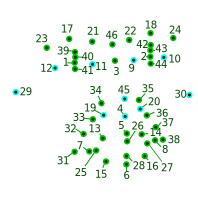
\includegraphics[width = 0.49 \columnwidth]{featureselection/TrackerPositions.pdf}
\caption[Manual division of tracker points into a flexible and rigid sets.]{Manual division of tracker points into a flexible and rigid sets. Flexible points are shown in green. Rigid points are shown in cyan. Humans have relatively little ability to move these rigid facial points relative to the skull.}
\label{FigureRigidTrackers}
\end{figure}

\begin{figure}[tb]
\centering
\begin{tabular}{ cc }
Agree & Question \\
\includegraphics[width = 0.49 \columnwidth]{featureselection/baragree.pdf} &
\includegraphics[width = 0.49 \columnwidth]{featureselection/barquestion.pdf} \\
\includegraphics[width = 0.49 \columnwidth]{featureselection/barthinking.pdf} & 
\includegraphics[width = 0.49 \columnwidth]{featureselection/barunderstand.pdf}\\
Thinking & Understand \\
\end{tabular}
\caption[Bar charts showing the normalised weights of tracking features for the four \ac{NVC} categories.]{Bar charts showing the normalised weights of tracking features for the four \ac{NVC} categories. Rigid and non-rigid trackers are shown as different colours, which indicate the relative importance of expression vs. head pose in recognition. The tracker ID numbers correspond to the numbering in Figure \ref{FigureRigidTrackers}. Results are from GBR culture, with person independent folds in feature selection. Visualisation areas have been averaged across test folds.}
\label{FigureFeatureWeightBarCharts}
\end{figure}

To investigate the relative importance of head pose when compared to the role expression, the trackers have been manually divided into rigid and non-rigid facial points. The manual division of trackers is shown in Figure \ref{FigureRigidTrackers}. However, it is possible to automatically separate points into rigid and flexible sets, as described by Del Bue \etal \cite{DelBue2005}. The normalised tracker weights for each of the four \ac{NVC} categories are shown in Figure \ref{FigureFeatureWeightBarCharts}. All \ac{NVC} categories have significant weights assigned to trackers on flexible parts of the face, which implies expression is significant for \ac{NVC} recognition. The weights assigned to rigid trackers are relatively low for \textit{question} \ac{NVC} and to some extent in \textit{thinking}. This suggests that these \ac{NVC} signals are largely conveyed by expression, with head pose having little importance. In contrast, the rigid tracker weights have higher weights in \textit{agree}, which suggests that head pose has a role in the automatic recognition process. This confirms our expectation that agreement is often expressed by the nodding of the head. The weightings also show that the trackers that have low weightings for all of the studied \ac{NVC} signals. The lowest weighted tracker overall was number 22, which corresponds to a part of the eyebrow. This may indicate a problem with this tracker or this area is redundant for recognizing these types of \ac{NVC} signals.

Although each tracker weight corresponds to a specific area of the face, it is difficult to form an overall impression of which areas of the face are involved, based on these bar charts. A better approach is to visualise the relevant areas in relation to an actual face. However, the visualisation process is complicated by the head pose. 
%If features for head pose where included in the visualisation, they would emphasis areas of the face which are rigid.
Head pose changes are not localised to an specific area of the face and should be removed. The head pose is generally encoded by the distance between two rigid points on the face. Facial deformations can either be encoded by distances which are either between rigid to flexible facial points or between flexible to flexible facial points.
%Position and weight information for rigid points was discarded. 
The remaining non-rigid points correspond to the flexible regions of the face and are responsible for facial deformations. The facial areas are based on a Voronoi tessellation of the face \cite{Dirichlet1850}, based on tracker positions on a manually selected frontal view of the face. The normalised weights of each tracked point are used to control the saturation of the local area in the image. Relevant areas are shown as normal saturation. Irrelevant areas are shown as desaturated, which makes the colour tend to pure white for low weights. This enables an intuitive way to visualise relevant areas for \ac{NVC} expression around the face.

\begin{figure}[tb]
\centering
\begin{tabular}{ cc }
Agree & Question \\
\includegraphics[width = 0.39 \columnwidth]{featureselection/visoutput-agree-crop-bng.png} &
\includegraphics[width = 0.39 \columnwidth]{featureselection/visoutput-question-crop-bng.png} \\
\includegraphics[width = 0.39 \columnwidth]{featureselection/visoutput-thinking-crop-bng.png} & 
\includegraphics[width = 0.39 \columnwidth]{featureselection/visoutput-understand-crop-bng.png}\\
Thinking & Understand \\
\end{tabular}
\caption[Visualising the areas of face used for \featureGeneration.]{Visualising the areas of face used for \featureGeneration. The face is segmented based on Voronoi tessellation. More saturated areas indicate the importance of an area, less saturated areas are not relevant for a particular \ac{NVC}. Results are from GBR culture, with person independent folds in feature selection. Visualisation areas have been averaged across test folds.}
\label{FigureFeatureSelectionVis}
\end{figure}

The results of the visualisation are shown in Figure \ref{FigureFeatureSelectionVis}. The clearest example of facial areas corresponding to our expectation is for \textit{thinking}. The eyes are prominently selected and gaze is already thought to play a role in this \ac{NVC}, as discussed in Section \ref{SectionVisualisingGaze}. The other features provide an indication into less well understood \ac{NVC}. The brow region seems important for \textit{question} \ac{NVC}. When intense examples of \textit{question} are viewed, there is generally consistent brow lowering (action unit 4) lasting for less than a second which occurs at or near the end of a question sentence (see Figure \ref{FigureBrowLoweringQuestion}). The feature selection seems to be using this behaviour as the basis for recognition. This connection between verbal questioning and brow lowering has not been previously reported in published research, although Ekman mentions unpublished experiments which found this association \cite{Ekman1979}. Brow raising and lowering has also been documented in sign language but in this context, the direction of raising or lowering has a distinct semantic meaning, depending on the type of question that is being asked \cite{Ekman1999}. For \textit{agree} and \textit{understand}, the areas selected are less specific but generally indicate that the eyes and mouth are involved and the brow area is not used. While the visualisation shows areas that are involved in \ac{NVC} recognition by \ac{ML}, it does not necessarily imply that humans use these areas for recognition, but shows that information is present in these areas. However, there is a strong possibility that humans also use this information during \ac{NVC} perception.

\begin{figure}[tb]
\includegraphics[width = 0.49 \columnwidth]{featureselection/question-clip_1HTGE8FuGw.jpg}
\includegraphics[width = 0.49 \columnwidth]{featureselection/question-clip_4bg18VX1W3.jpg} \\
\caption{Brow lowering (action unit 4), lasting for less than a second, often occurs at or near the end of a question sentence.}
\label{FigureBrowLoweringQuestion}
\end{figure}

This approach could be improved by additional trackers, would would improve the spatial resolution of the visualisation. %Determining the relative importance of head pose might also be useful, particularly for \textit{agree} which can involve head nodding. %Visualisation of feature selection can provide clues as to how human perception operates.

\section{Applying Feature Selection to the Mind Reading Corpus}
\label{SectionMindReadingFeatureSelection}

Classification of mental states in the Mind Reading corpus was previously discussed in Section \ref{SectionMindReading}. This section applies feature selection to the algorithmic geometric features in an attempt to improve classification performance. The motivation is the save as in the case of TwoTalk: the feature vector contains irrelevant or redundant information which can reduce the performance of recognition. The experimental arrangement used is the same as described in Section \ref{SectionMindReading}, except for only a subset of features are used, as determined by Algorithm \ref{AlgFeatureSelectOverview}. Because cross validation evaluation is performed on a leave-one-clip-out basis, it is not computationally feasible to perform a separate feature selection for each of the 174 folds. In this case, feature selection is conducted on a two fold basis on the entire corpus. As the feature selection removes features by \ac{SBE}, the performance based on two fold classification accuracy rises. The change in performance during the \ac{SBE} process is shown in Figure \ref{FigureMindReadingPerfFeatureSbe}. The resultant masks are then evaluated using the standard level-one-clip-out; the classification accuracy of this is shown in Figure \ref{FigureMindReadingSbeTestPerf}. As usual, the performance gradually increases as unnecessary or detrimental features are removed, before a sudden reduction in performance. Peak performance for the feature selection occurs for between 50 and 90 feature components. A set of 88 feature components is manually selected, based on it having the best classification accuracy. The number of features removed at each stage is as follows:

\begin{gather}
\label{EquationNumFeaturesToRemoveMindReading}
\numToRemoveInMask = \begin{cases}
4 : \numFeaturesInMask > 1000 \\
2 : \numFeaturesInMask > 500, \numFeaturesInMask \le 1000 \\
1 : \numFeaturesInMask \le 500
\end{cases}
\end{gather}

This removes features more slowly than in the previous section, which should help prevent useful features being eliminated. However, this results in the system being evaluated at more stages during the \ac{SBE} process.

\begin{figure}
\centering
\includegraphics[width = 0.8 \columnwidth]{featureselection/mindreading-fs.pdf}
\caption{Classification accuracy of two-fold cross validation on the Mind Reading corpus as features are eliminated by \ac{SBE}.}
\label{FigureMindReadingPerfFeatureSbe}
\end{figure}

\begin{figure}
\centering
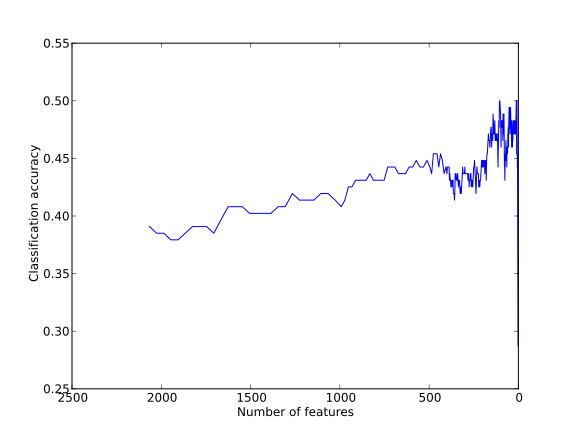
\includegraphics[width = 0.8 \columnwidth]{featureselection/mindreading-test.pdf}
\caption{Classification accuracy of level-one-clip-out cross validation on the Mind Reading corpus as features are eliminated by \ac{SBE}, based on the previously selected feature sets.}
\label{FigureMindReadingSbeTestPerf}
\end{figure}

\begin{figure}
\centering
\includegraphics[width = 0.8 \columnwidth]{featureselection/MindReadingFeatureSelectPerf.png}
\caption[Performance of various classification methods based on the Mind Reading Corpus.]{Performance of various classification methods based on the Mind Reading Corpus. Orange corresponds to algorithmic geometric features without feature selection (method described in Section \ref{SectionMindReading}). Green corresponds to the algorithmic geometric feature selection method proposed in this section, with 88 components. Yellow corresponds to el Kaliouby and Robinson \cite{ElKaliouby2004}. Chance prediction performance is 17\%.}
\label{FigureMindReadingAlgFs}
\end{figure}

\begin{table}[tb]
\centering
\caption[Confusion matrix of mental state classification using geometric algorithmic features with feature selection on the Mind Reading corpus.]{Confusion matrix of mental state classification using geometric algorithmic features with feature selection on the Mind Reading corpus. Feature selection resulted in a set of 88 feature components which are more effective at classification.}
\scriptsize 
\begin{tabular}{ c || c | c | c | c | c | c || c  }
\hline
mental state&agreeing&concentrating&disagreeing&interested&thinking&unsure&accuracy\\
\hline
agreeing	&\textbf{20}	&0	&4	&2	&5	&5	&55.6\%\\
concentrating	&0	&\textbf{0}	&2	&7	&3	&6	&0.0\%\\
disagreeing	&7	&0	&\textbf{8}	&2	&3	&4	&33.3\%\\
interested	&2	&2	&0	&\textbf{20}	&2	&4	&66.7\%\\
thinking	&5	&3	&2	&2	&\textbf{21}	&3	&58.3\%\\
unsure		&1	&2	&2	&2	&5	&\textbf{18}	&60.0\%\\
mean		&	&	&	&	&	&	&\textbf{45.6}\%\\
\end{tabular}
\normalsize
\label{TableMindReadingAlgFs}
\end{table}

The use of feature selection results in a significant performance increase but is still not as effective as el Kaliouby and Robinson \cite{ElKaliouby2004}. Classification for \textit{concentrating} is worse than chance classification and is often mislabelled as \textit{interested} or \textit{unsure}, which are arguable closely related to \textit{concentrating}. There are less examples of \textit{concentrating} in the corpus, which may be a factor in poor recognition performance for this class. Other reasons for the lower performance include:

\begin{itemize}
 \item Acted behaviour is more intense and more consistent than spontaneous behaviour. This may be exploited by the temporal model used by el Kaliouby and Robinson to achieve a better result.
 \item \ac{NVC} and mental states are different concepts. The proposed system was developed for \ac{NVC} and el Kaliouby and Robinson's system was developed to address the Mind Reading corpus.
 \item There is less video data available for each class and more subjects in the Mind Reading corpus, which may affect which method is suitable. Specifically, the proposed method uses subject specific normalisation which can require a significant amount of data to reach a stable and robust model of facial behaviour.
 \item el Kaliouby and Robinson discarded video clips that were not tracked, while we consider all videos, which is a harder problem.
 \item The \featureGeneration technique used by each method is different, which may encode relevant information that is missed by other \featureGeneration approaches. Although the \textit{geometric-h} heuristic features are based on el Kaliouby and Robinson, it is not the same. They use appearance features that focus on mouth opening and teeth visible, which may be useful in distinguishing some of the classes.
 \item Feature selection on geometric algorithmic features was conducted based on the performance of all classes. However, it may be more effective to have a one-vs-one class basis for feature selection, to better isolate features that distinguish each class.
\end{itemize}

\section{Conclusion}

%As seen in the previous chapter, features generated based on tracker distances can encode facial deformation as a step in \ac{NVC} recognition. 
Geometric features used in the previous chapter contain a great deal of redundant and irrelevant components. This chapter describes an \ac{SBE} based method to find a subset of features that are relevant for a specific \ac{NVC} signal. This removes feature components that are not relevant for \ac{NVC} recognition and this results in a significant performance increase. The feature subset is then visualised to show the facial areas used by the automatic system. This provides evidence of which facial areas are involved in the expression of each \ac{NVC} signal. Knowing the areas of the face used for \ac{NVC} can suggest feature types that better encode these local areas, avoids computation of irrelevant or redundant features, as well as improving our understanding of human behaviour.

The areas of the face that are used by the system either correspond to the expected areas, or for \ac{NVC} signals that are less well understood, they give an indication as to the facial areas that are involved. The areas used for each \ac{NVC} are different, which implies that the feature selection has isolated feature components that are specific to each \ac{NVC}. Thinking is known to involve gaze aversion and this is clearly seen in that feature components that encode eye movement are retained by the feature selection process. Based on reviewing corpus videos, it was manually observed that a sentence ending with a question is often accompanied by a brief brow lowering and this is also consistent with the visualisation of questioning \ac{NVC}.

\ac{SBE} feature selection was based on multiple folds of the seen data. Using folds that were either person-independent or person-dependent did not make a significant performance difference. The termination of the \ac{SBE} process was based on the peak performance of the training data used in the optimisation. This does not select the optimal number of features but it still resulted in a significant performance increase. If a system can be manually tuned, a slightly better performance can be achieved but the number of features that is optimal depends on the specific \ac{NVC}.

The visualisation of the feature selection subsets used annotation data from a single culture. It may be possible to investigate whether other cultures use different areas of the face for \ac{NVC} perception, based on feature selection. Gaze patterns are culturally dependent for emotion recognition \cite{Jack2009}. However, humans may be using different areas of the face for recognition, compared to an automatic system. This may be due to the feature extraction process not being as comprehensive as human perception. The areas used by an automatic system may provide indirect clues as to the way human perception operates. This cross cultural visualisation is not attempted in this thesis, because this would require a larger video corpus, more comprehensive facial encoding and additional annotation data to provide a reliable result.

Head pose has a role in \ac{NVC} but the visualisation in this chapter is focused on local facial deformations. The features are only considered as simplistic temporal variations. The temporal encoding currently considers an entire clip, so cannot temporally localise relevant motion in \ac{NVC} expression. However, with more detailed temporal encoding, which might consider variation in a sliding window, a particular time and area of the face could be identified as important for \ac{NVC} automatic regression. The feature selection framework also might provide a framework to extend the existing automatic system to other feature types. Considering many different areas of the face (or holistic facial features) over multiple time scales and temporal offsets will result in a vast number of potential features. For this reason, techniques that are suitable for spotting patterns in large data sets, such as data mining, may be relevant to facial analysis. %Also techniques that separate relevant features from irrelevant ones, such as feature selection, will reduce the quantity of features to a practical level.

The feature selection method presented here is a simple but computationally intensive approach. The removal of many features during the early iterations was necessary to make the approach practical but the performance implications of this approximation are not well understood. Other feature selection methods may be investigated to reduce the computation requirements and improve performance.

%The final chapter draws broad conclusions for the overall thesis and discusses the work in context.
